\begin{frame}
\frametitle{CERN \& LHC}
\begin{center}
\begin{tikzpicture}[scale=.95]
\node[anchor=south west,inner sep=0] at (0,0) {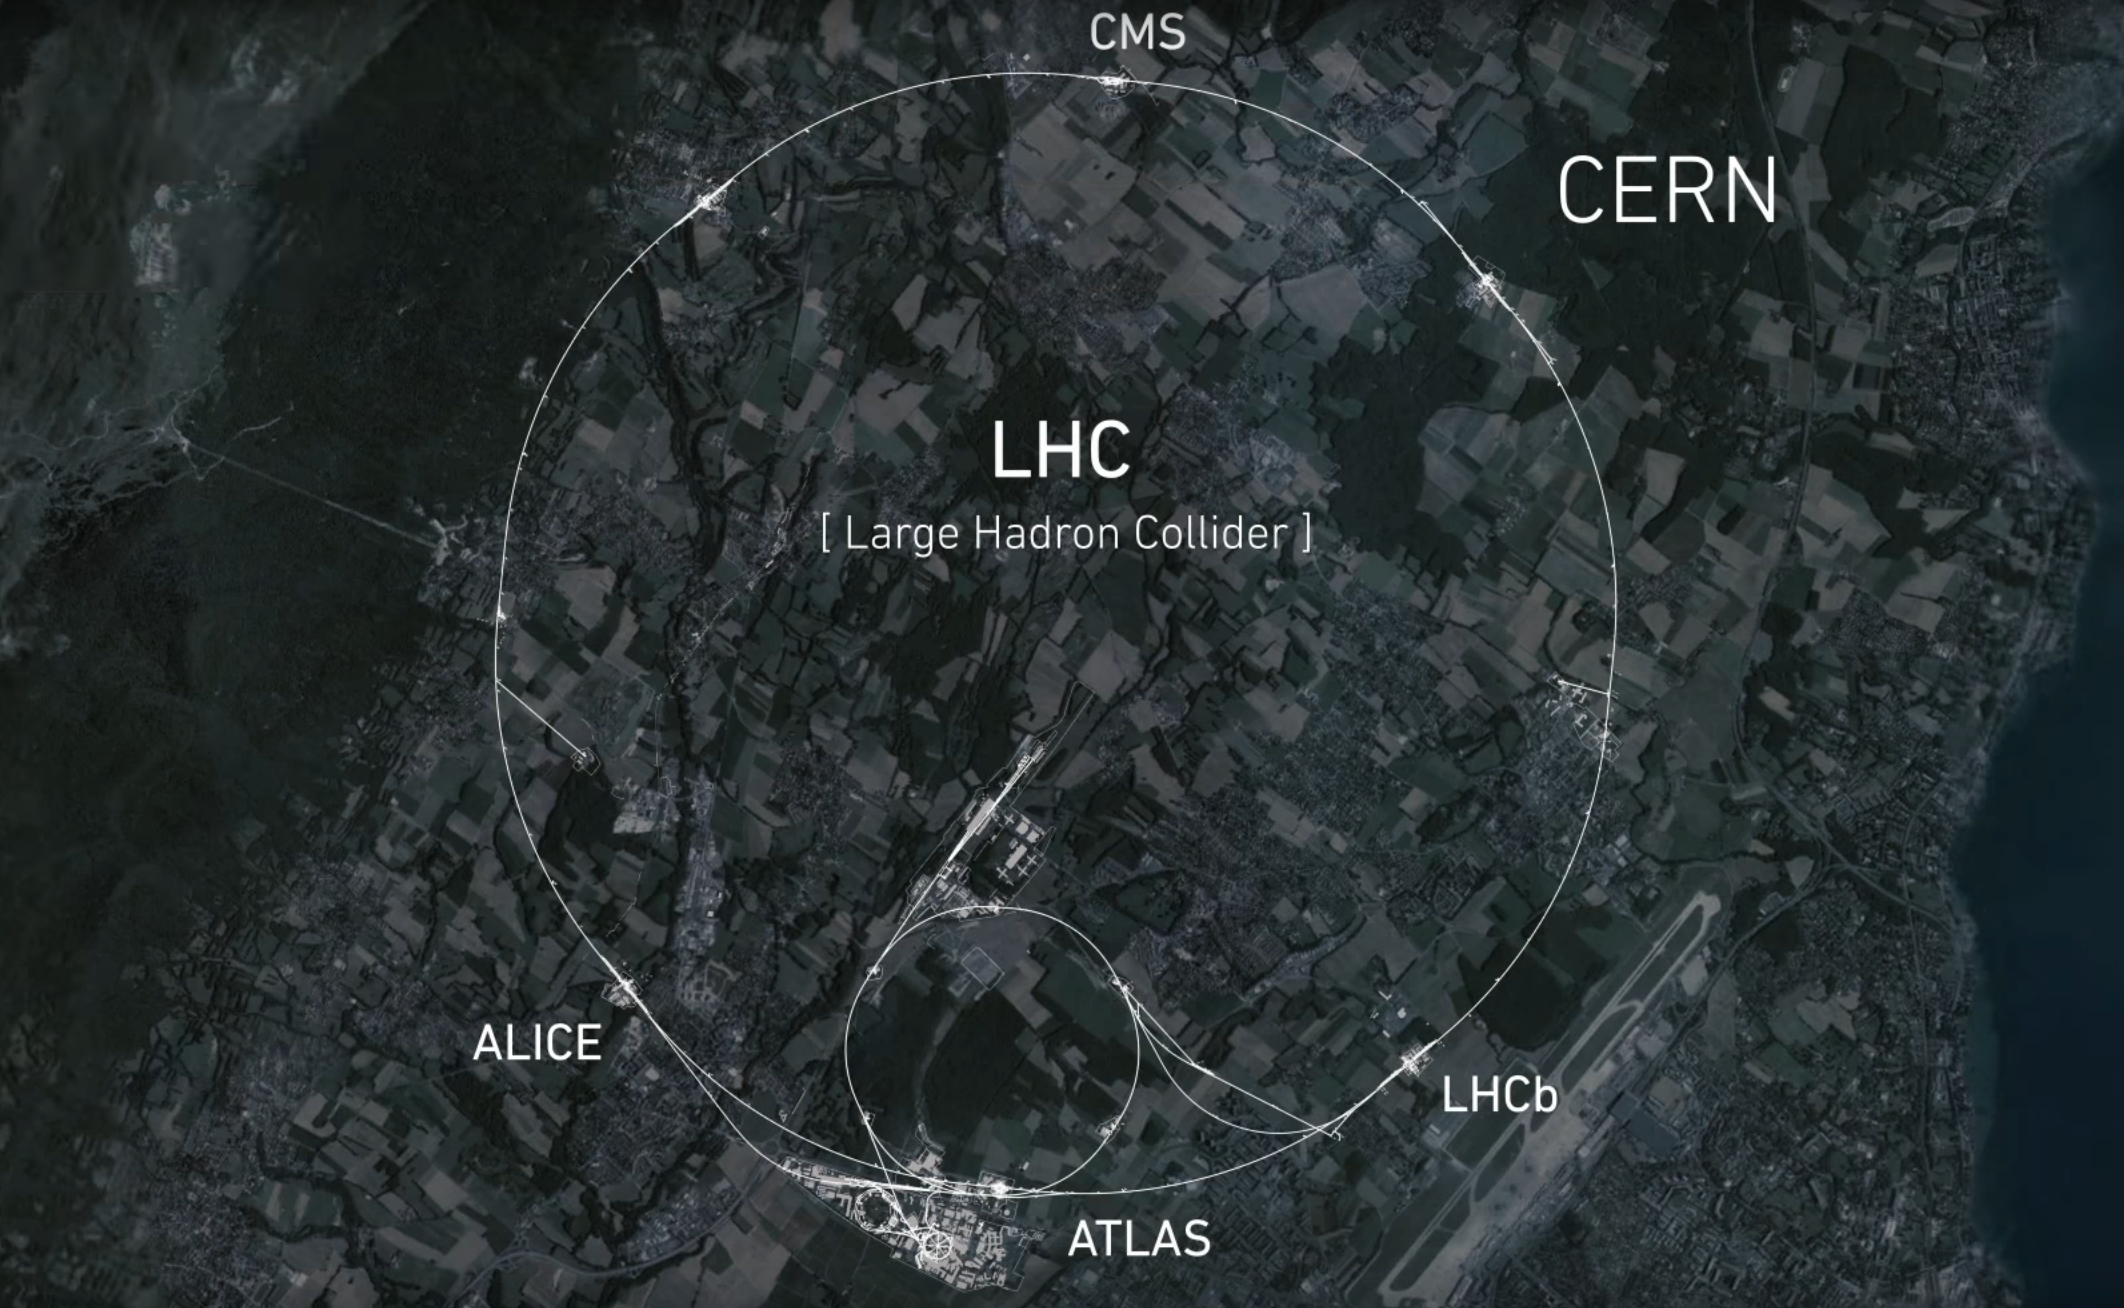
\includegraphics[height=6.65cm]{\PhDthesisdir/plots_and_images/CERN_and_LHC/LHC_map2.png}};
%\draw [ultra thick, ltcolorred] (5.65,3.6) circle (3) ; %LHC
%\draw [ultra thick, ltcolorred] (5.325,1.375) circle (.775) ; % SPS
%\draw [ultra thick, ltcolorred] (5.025,0.34) circle (.075) ; % PS
%\fill [ltcolorred] (4.925,0.375) circle (.025) ; % Booster
%\draw [thick, ltcolorred] (4.925,0.375) --+ (-85:.1) ; % LINAC2
\node[anchor=south west,inner sep=0] at (.75,5) {
\includegraphics[height=1cm]{\PhDthesisdir/plots_and_images/misc_for_slides/flag-france.jpg}};
\node[anchor=south west,inner sep=0] at (9.5,.5) {
\includegraphics[height=1cm]{\PhDthesisdir/plots_and_images/misc_for_slides/flag-suisse.png}};
\end{tikzpicture}
\end{center}
\end{frame}

\begin{frame}\addtocounter{framenumber}{-1}
\frametitle{LHC}
\begin{center}
\begin{tikzpicture}[scale=.95]
\node[anchor=south west,inner sep=0] at (0,0) {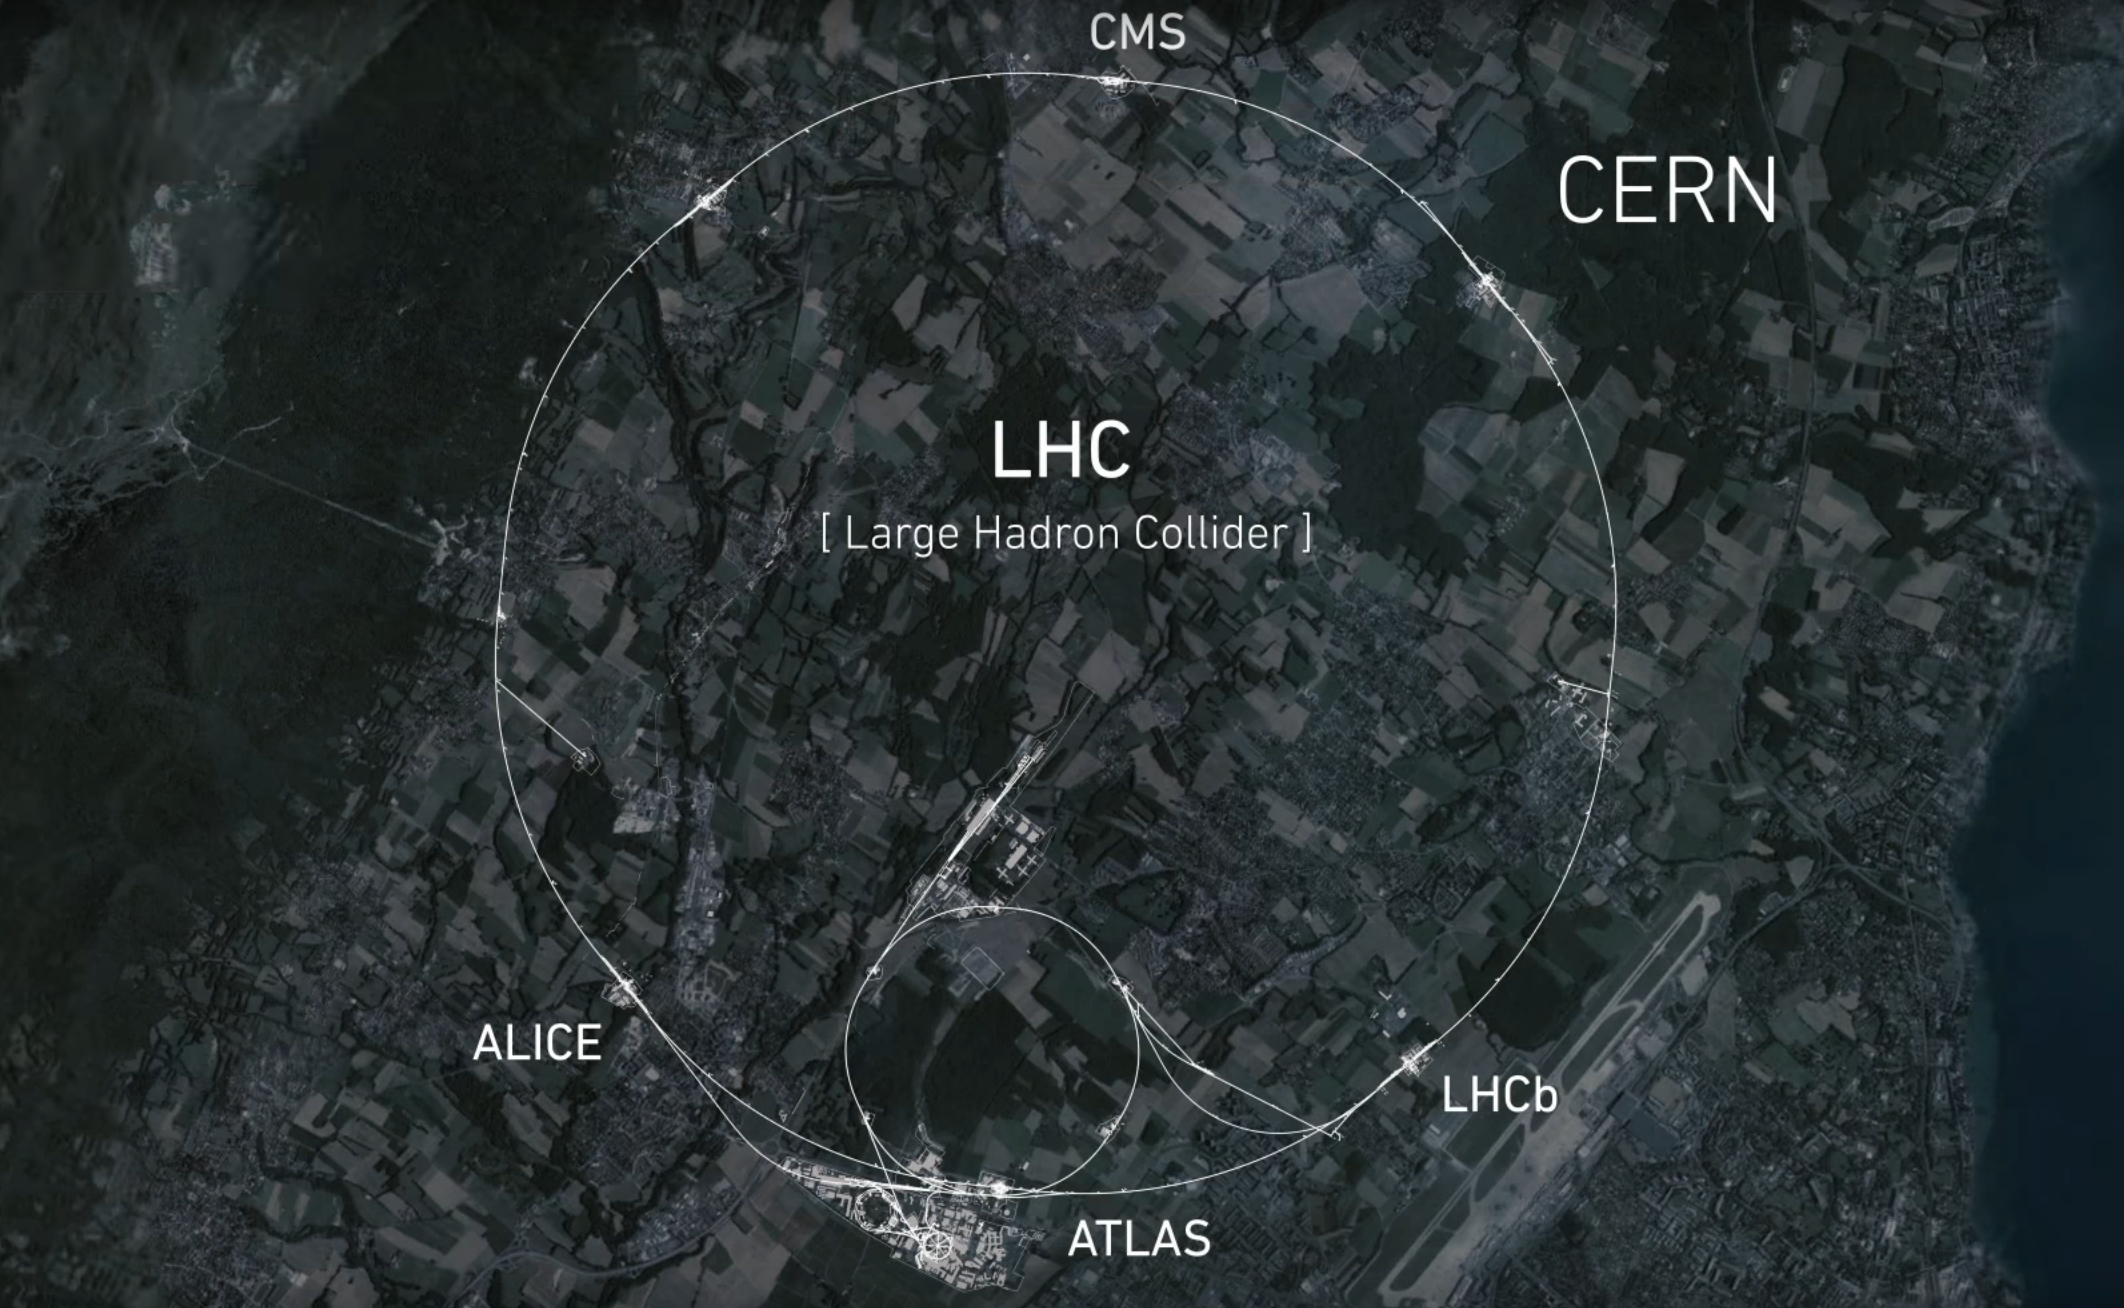
\includegraphics[height=6.65cm]{\PhDthesisdir/plots_and_images/CERN_and_LHC/LHC_map2.png}};
\draw [ultra thick, ltcolorred] (5.65,3.6) circle (3) ; %LHC
%\draw [ultra thick, ltcolorred] (5.325,1.375) circle (.775) ; % SPS
%\draw [ultra thick, ltcolorred] (5.025,0.34) circle (.075) ; % PS
%\fill [ltcolorred] (4.925,0.375) circle (.025) ; % Booster
%\draw [thick, ltcolorred] (4.925,0.375) --+ (-85:.1) ; % LINAC2
\end{tikzpicture}
\end{center}
\end{frame}

\begin{frame}\addtocounter{framenumber}{-1}
\frametitle{LINAC2 (\SI{50}{\MeV})}
\begin{center}
\begin{tikzpicture}[scale=.95]
\node[anchor=south west,inner sep=0] at (0,0) {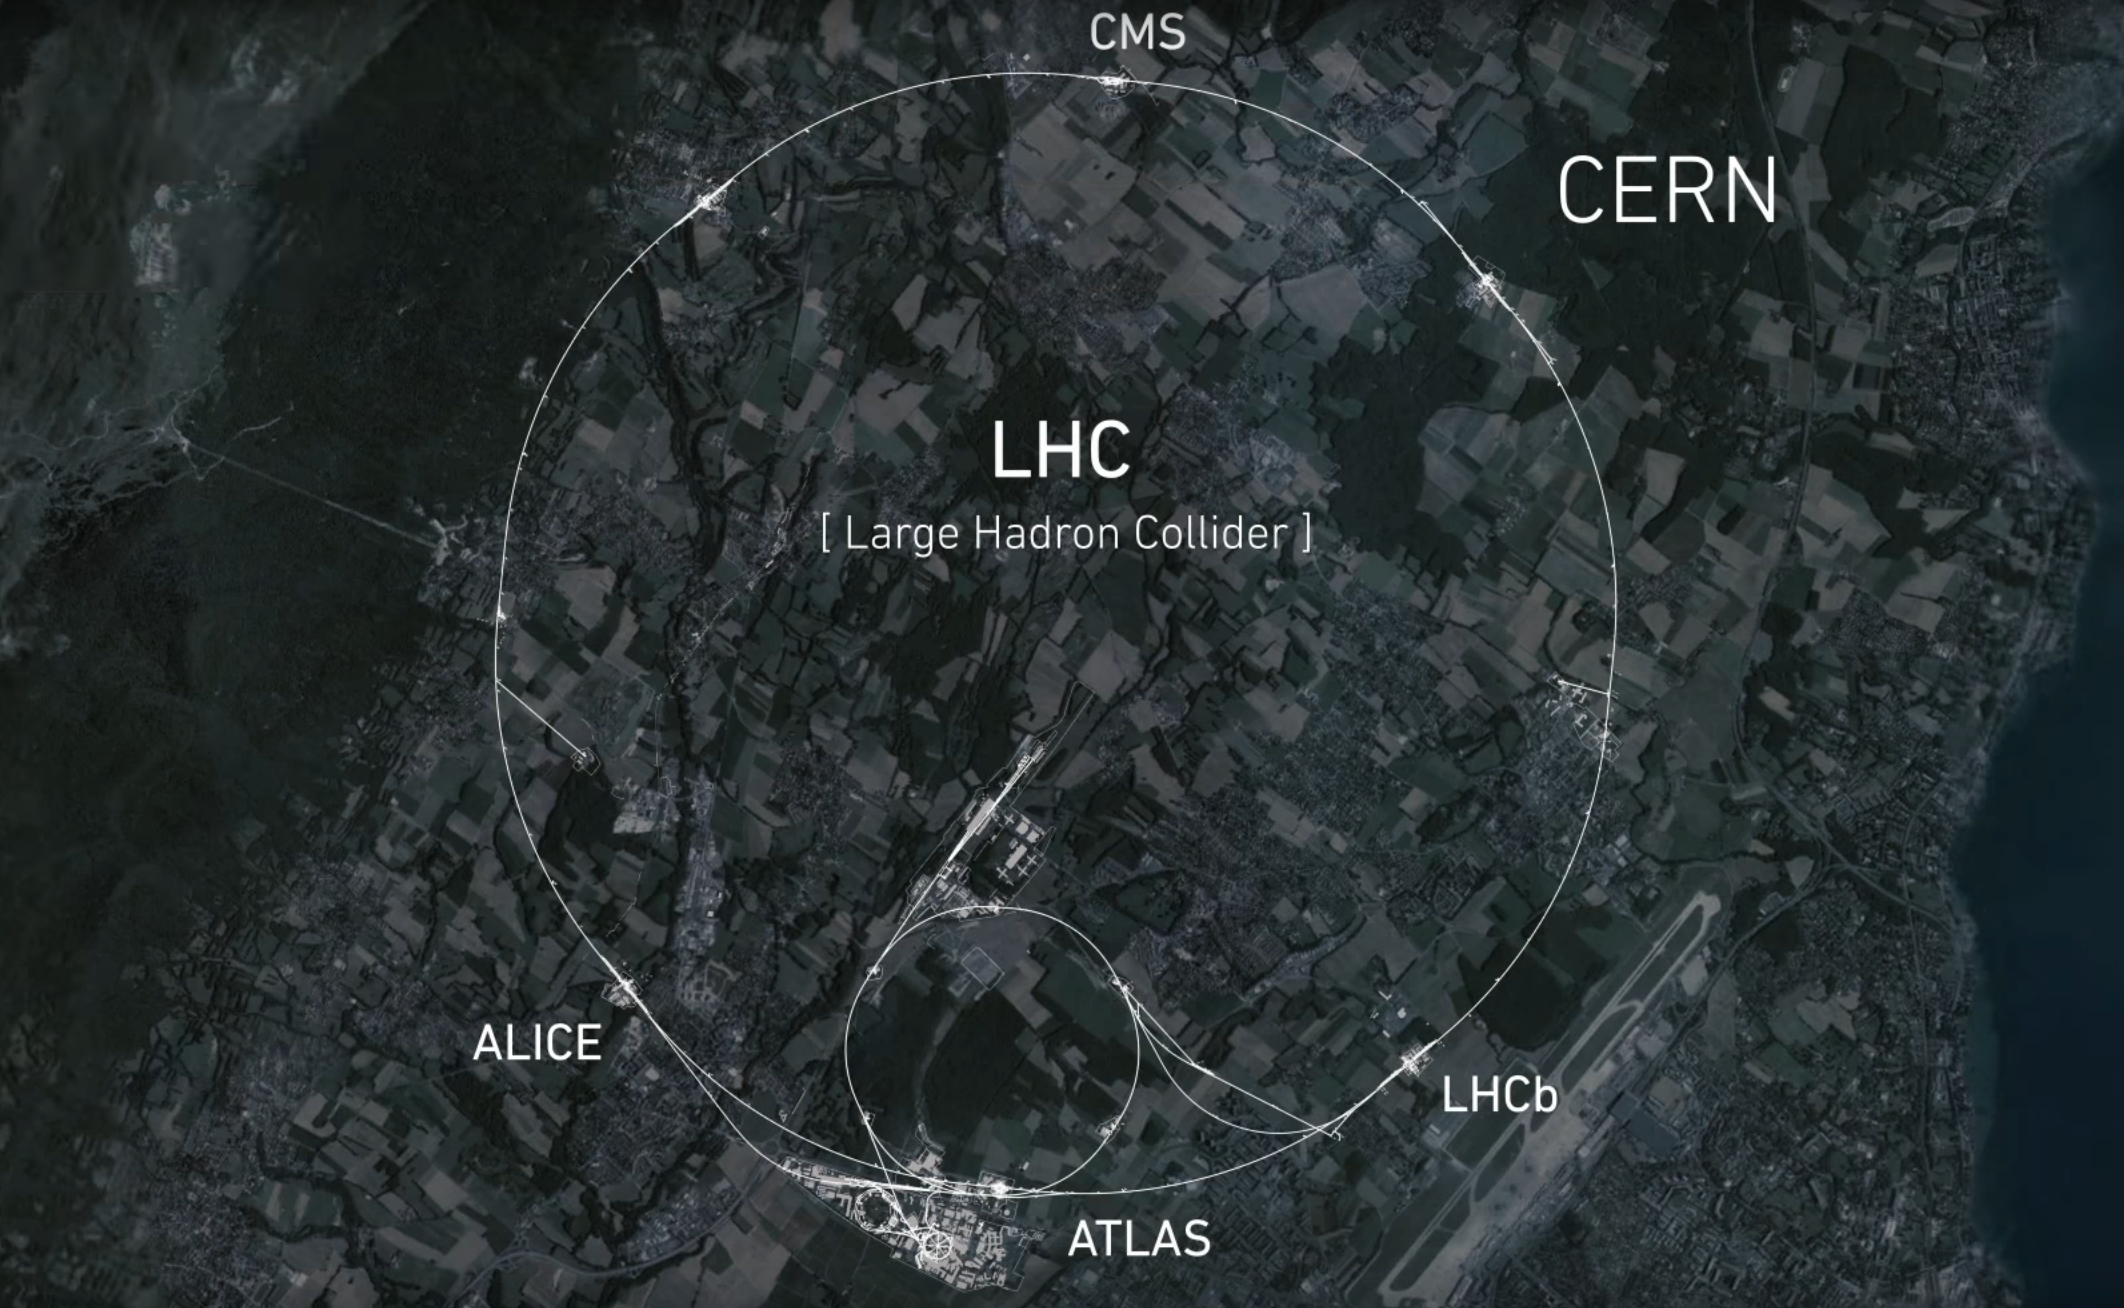
\includegraphics[height=6.65cm]{\PhDthesisdir/plots_and_images/CERN_and_LHC/LHC_map2.png}};
%\draw [ultra thick, ltcolorred] (5.65,3.6) circle (3) ; %LHC
%\draw [ultra thick, ltcolorred] (5.325,1.375) circle (.775) ; % SPS
%\draw [ultra thick, ltcolorred] (5.025,0.34) circle (.075) ; % PS
%\fill [ltcolorred] (4.925,0.375) circle (.025) ; % Booster
\draw [thick, ltcolorred] (4.925,0.375) --+ (-85:.1) ; % LINAC2
\draw [ultra thick, ltcolorred, latex-] (4.925,0.375) --+ (170:3) ;
\end{tikzpicture}
\end{center}
\end{frame}

\begin{frame}\addtocounter{framenumber}{-1}
\frametitle{Booster (1972, \SI{157}{\meter}, \SI{1.4}{\GeV})}
\begin{center}
\begin{tikzpicture}[scale=.95]
\node[anchor=south west,inner sep=0] at (0,0) {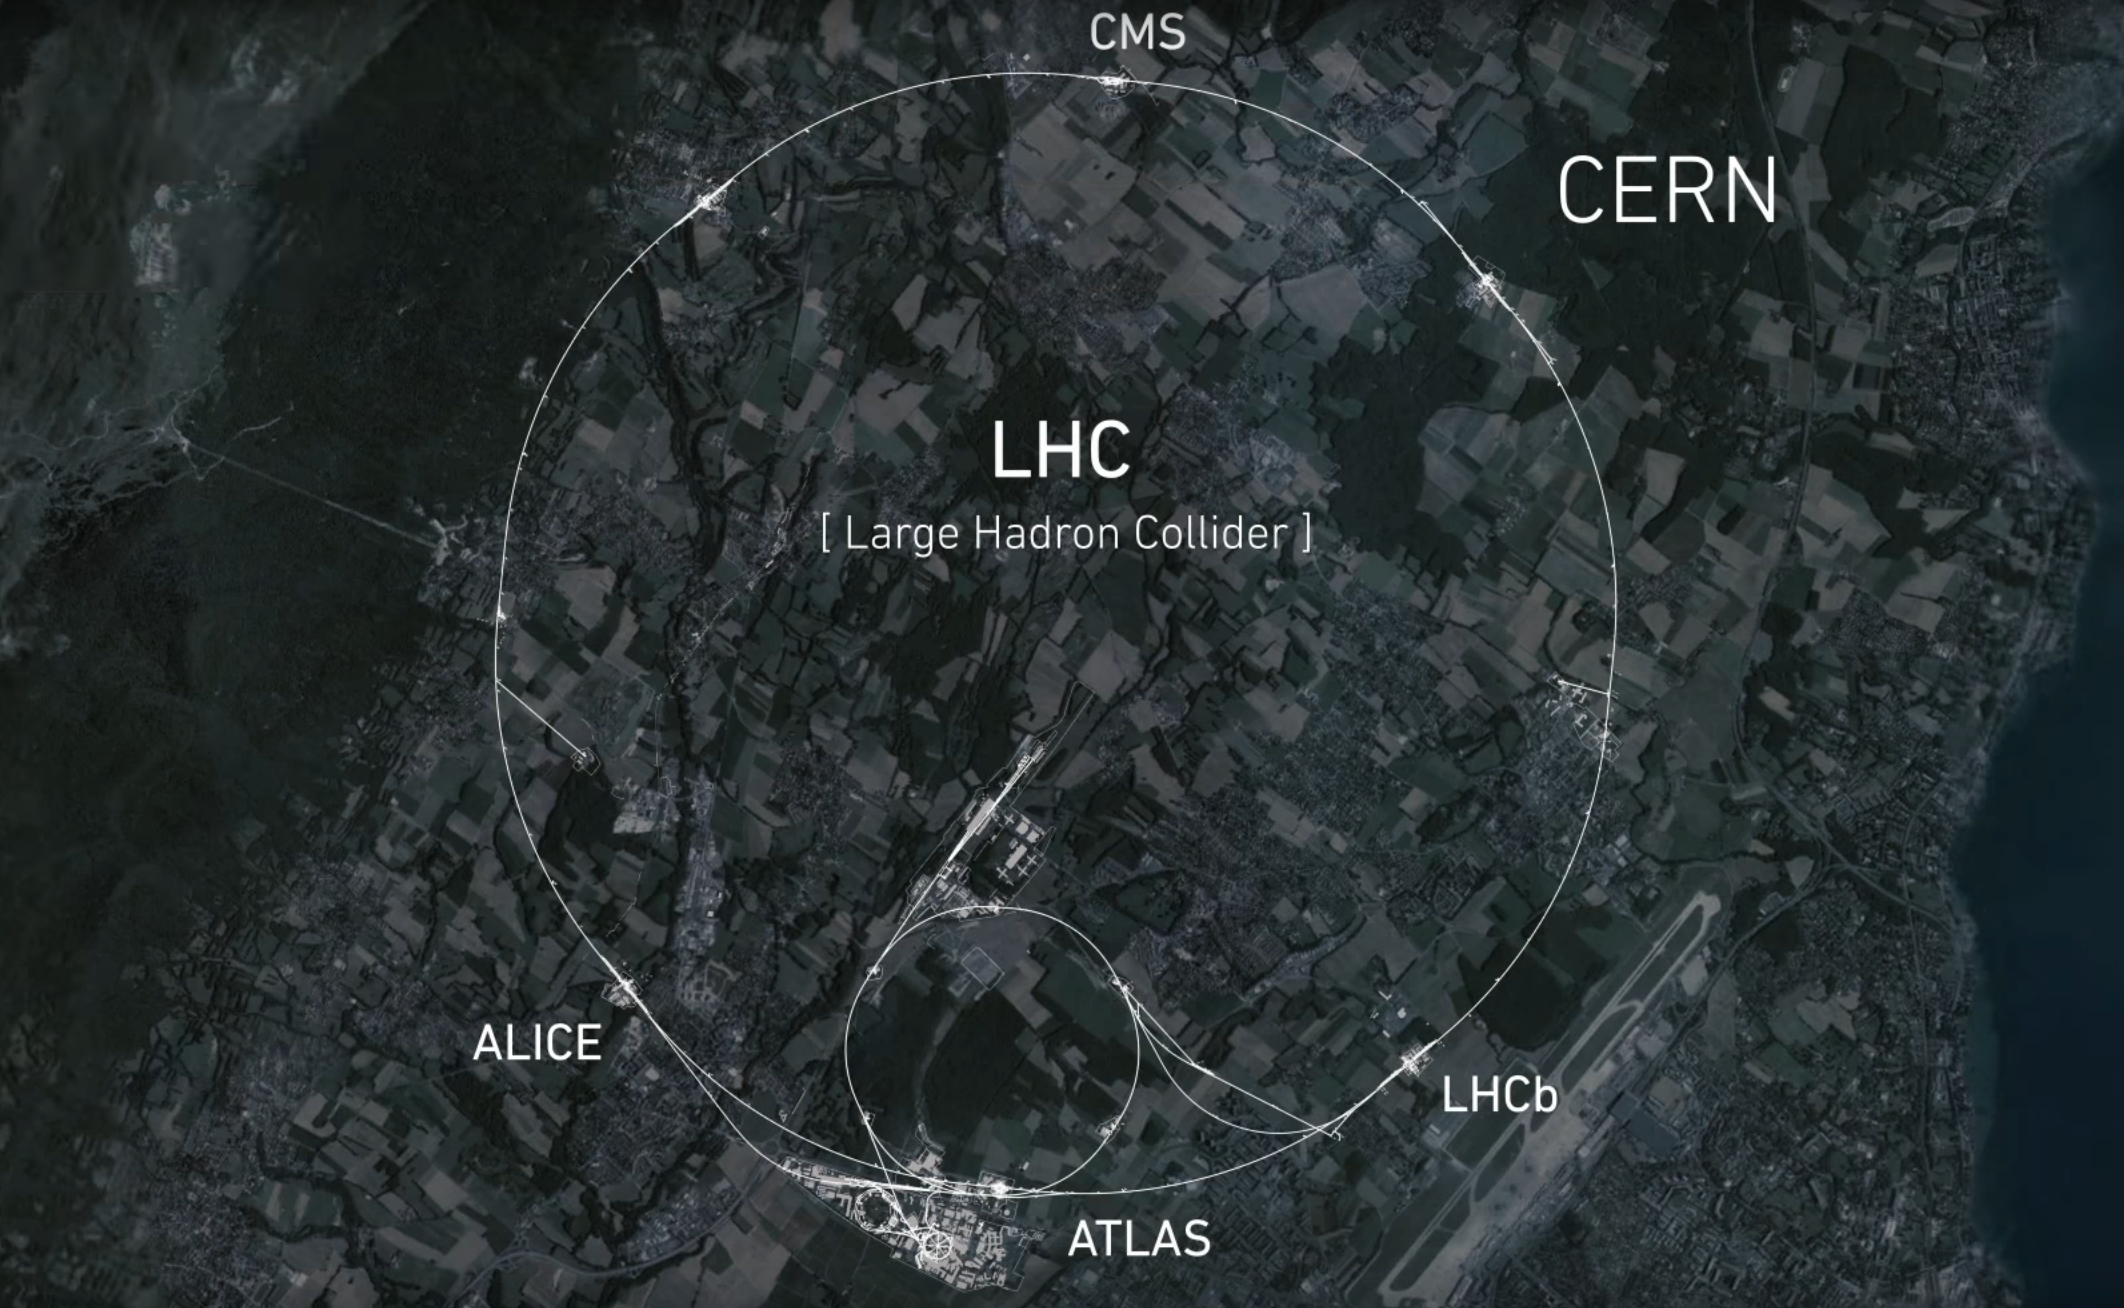
\includegraphics[height=6.65cm]{\PhDthesisdir/plots_and_images/CERN_and_LHC/LHC_map2.png}};
%\draw [ultra thick, ltcolorred] (5.65,3.6) circle (3) ; %LHC
%\draw [ultra thick, ltcolorred] (5.325,1.375) circle (.775) ; % SPS
%\draw [ultra thick, ltcolorred] (5.025,0.34) circle (.075) ; % PS
\fill [ltcolorred] (4.925,0.375) circle (.025) ; % Booster
%\draw [thick, ltcolorred] (4.925,0.375) --+ (-85:.1) ; % LINAC2
\draw [ultra thick, ltcolorred, latex-] (4.925,0.375) --+ (170:3) ;
\end{tikzpicture}
\end{center}
\end{frame}

\begin{frame}\addtocounter{framenumber}{-1}
\frametitle{PS (1959, \SI{628}{\meter}, \SI{25}{\GeV})}
\begin{center}
\begin{tikzpicture}[scale=.95]
\node[anchor=south west,inner sep=0] at (0,0) {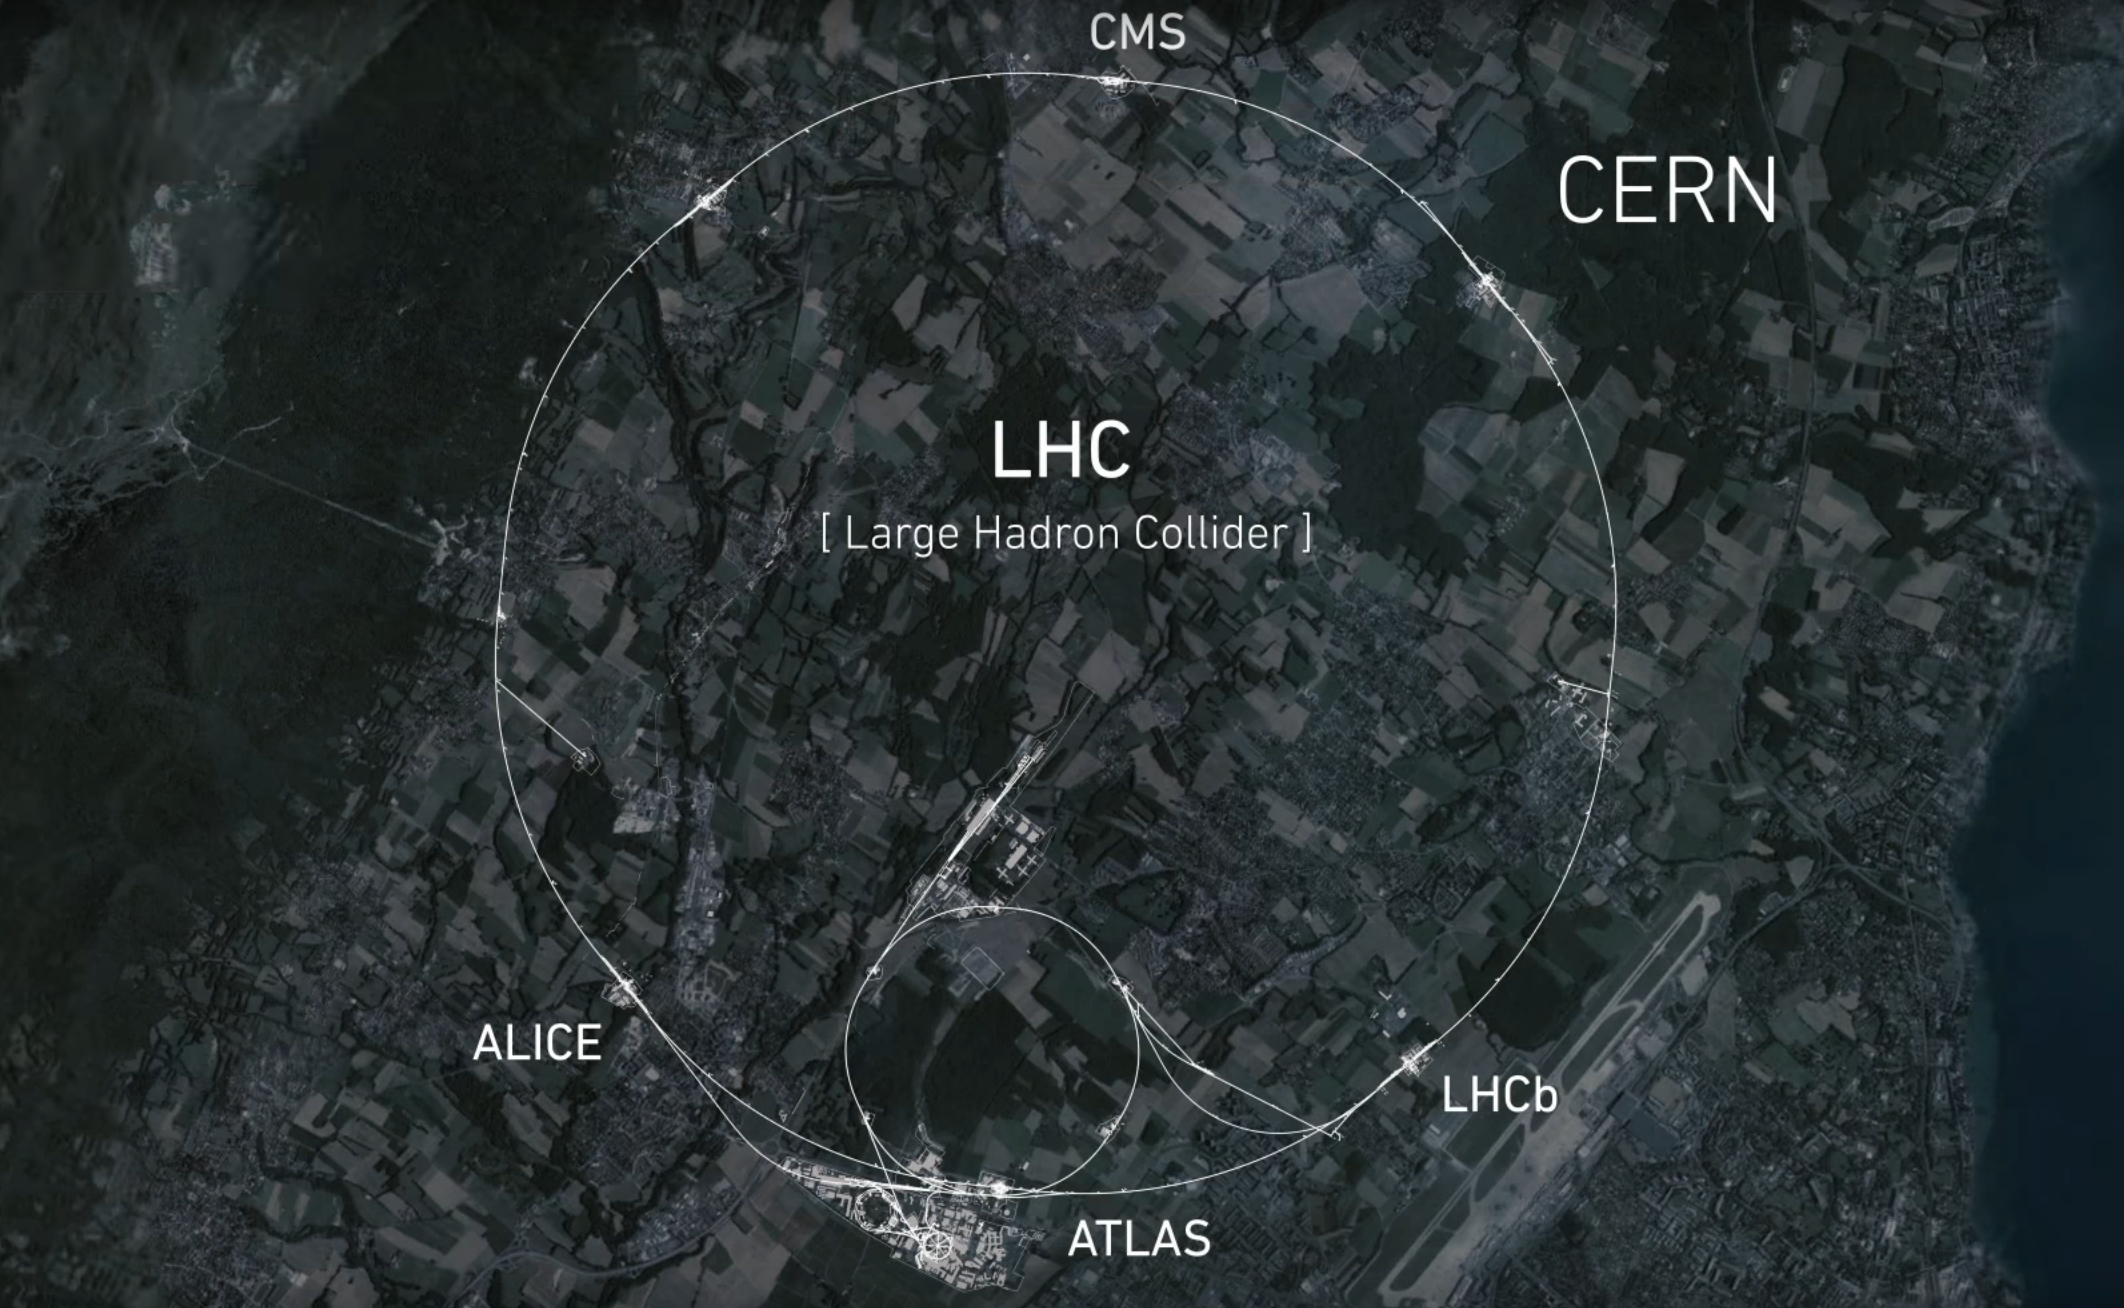
\includegraphics[height=6.65cm]{\PhDthesisdir/plots_and_images/CERN_and_LHC/LHC_map2.png}};
%\draw [ultra thick, ltcolorred] (5.65,3.6) circle (3) ; %LHC
%\draw [ultra thick, ltcolorred] (5.325,1.375) circle (.775) ; % SPS
\draw [ultra thick, ltcolorred] (5.025,0.34) circle (.075) ; % PS
%\fill [ltcolorred] (4.925,0.375) circle (.025) ; % Booster
%\draw [thick, ltcolorred] (4.925,0.375) --+ (-85:.1) ; % LINAC2
\draw [ultra thick, ltcolorred, latex-] (4.925,0.375) --+ (170:3) ;
\end{tikzpicture}
\end{center}
\end{frame}

\begin{frame}\addtocounter{framenumber}{-1}
\frametitle{SPS (1976, \SI{7}{\kilo\meter}, \SI{450}{\GeV})}
\begin{center}
\begin{tikzpicture}[scale=.95]
\node[anchor=south west,inner sep=0] at (0,0) {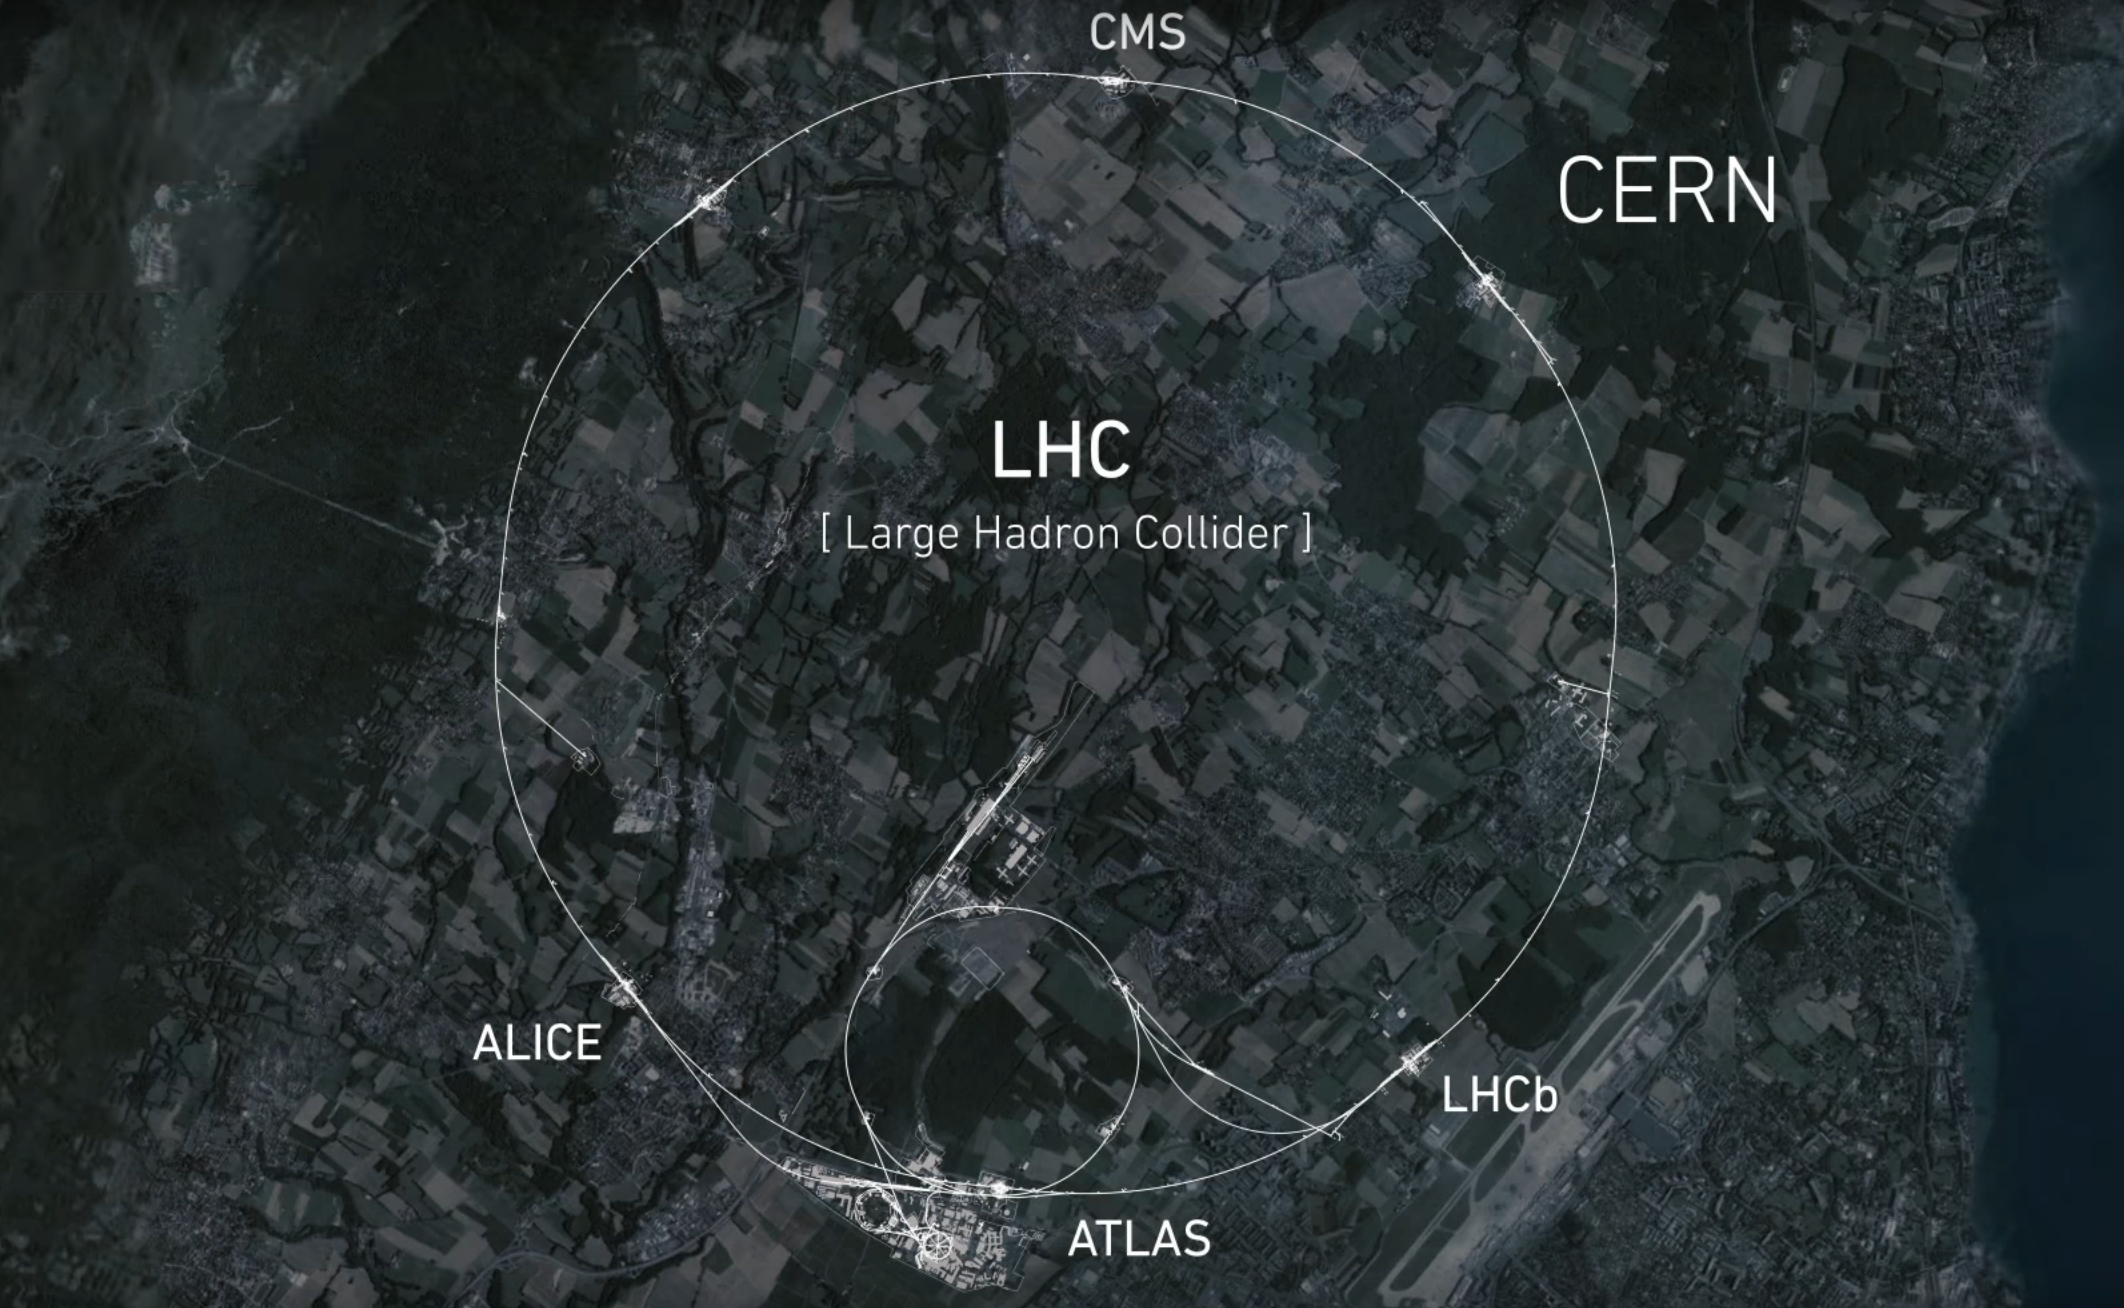
\includegraphics[height=6.65cm]{\PhDthesisdir/plots_and_images/CERN_and_LHC/LHC_map2.png}};
%\draw [ultra thick, ltcolorred] (5.65,3.6) circle (3) ; %LHC
\draw [ultra thick, ltcolorred] (5.325,1.375) circle (.775) ; % SPS
%\draw [ultra thick, ltcolorred] (5.025,0.34) circle (.075) ; % PS
%\fill [ltcolorred] (4.925,0.375) circle (.025) ; % Booster
%\draw [thick, ltcolorred] (4.925,0.375) --+ (-85:.1) ; % LINAC2
\end{tikzpicture}
\end{center}
\end{frame}

\begin{frame}\addtocounter{framenumber}{-1}
\frametitle{LHC (2008, \SI{27}{\kilo\meter}, $2\times\SI{7}{\TeV}$)}
\begin{center}
\begin{tikzpicture}[scale=.95]
\node[anchor=south west,inner sep=0] at (0,0) {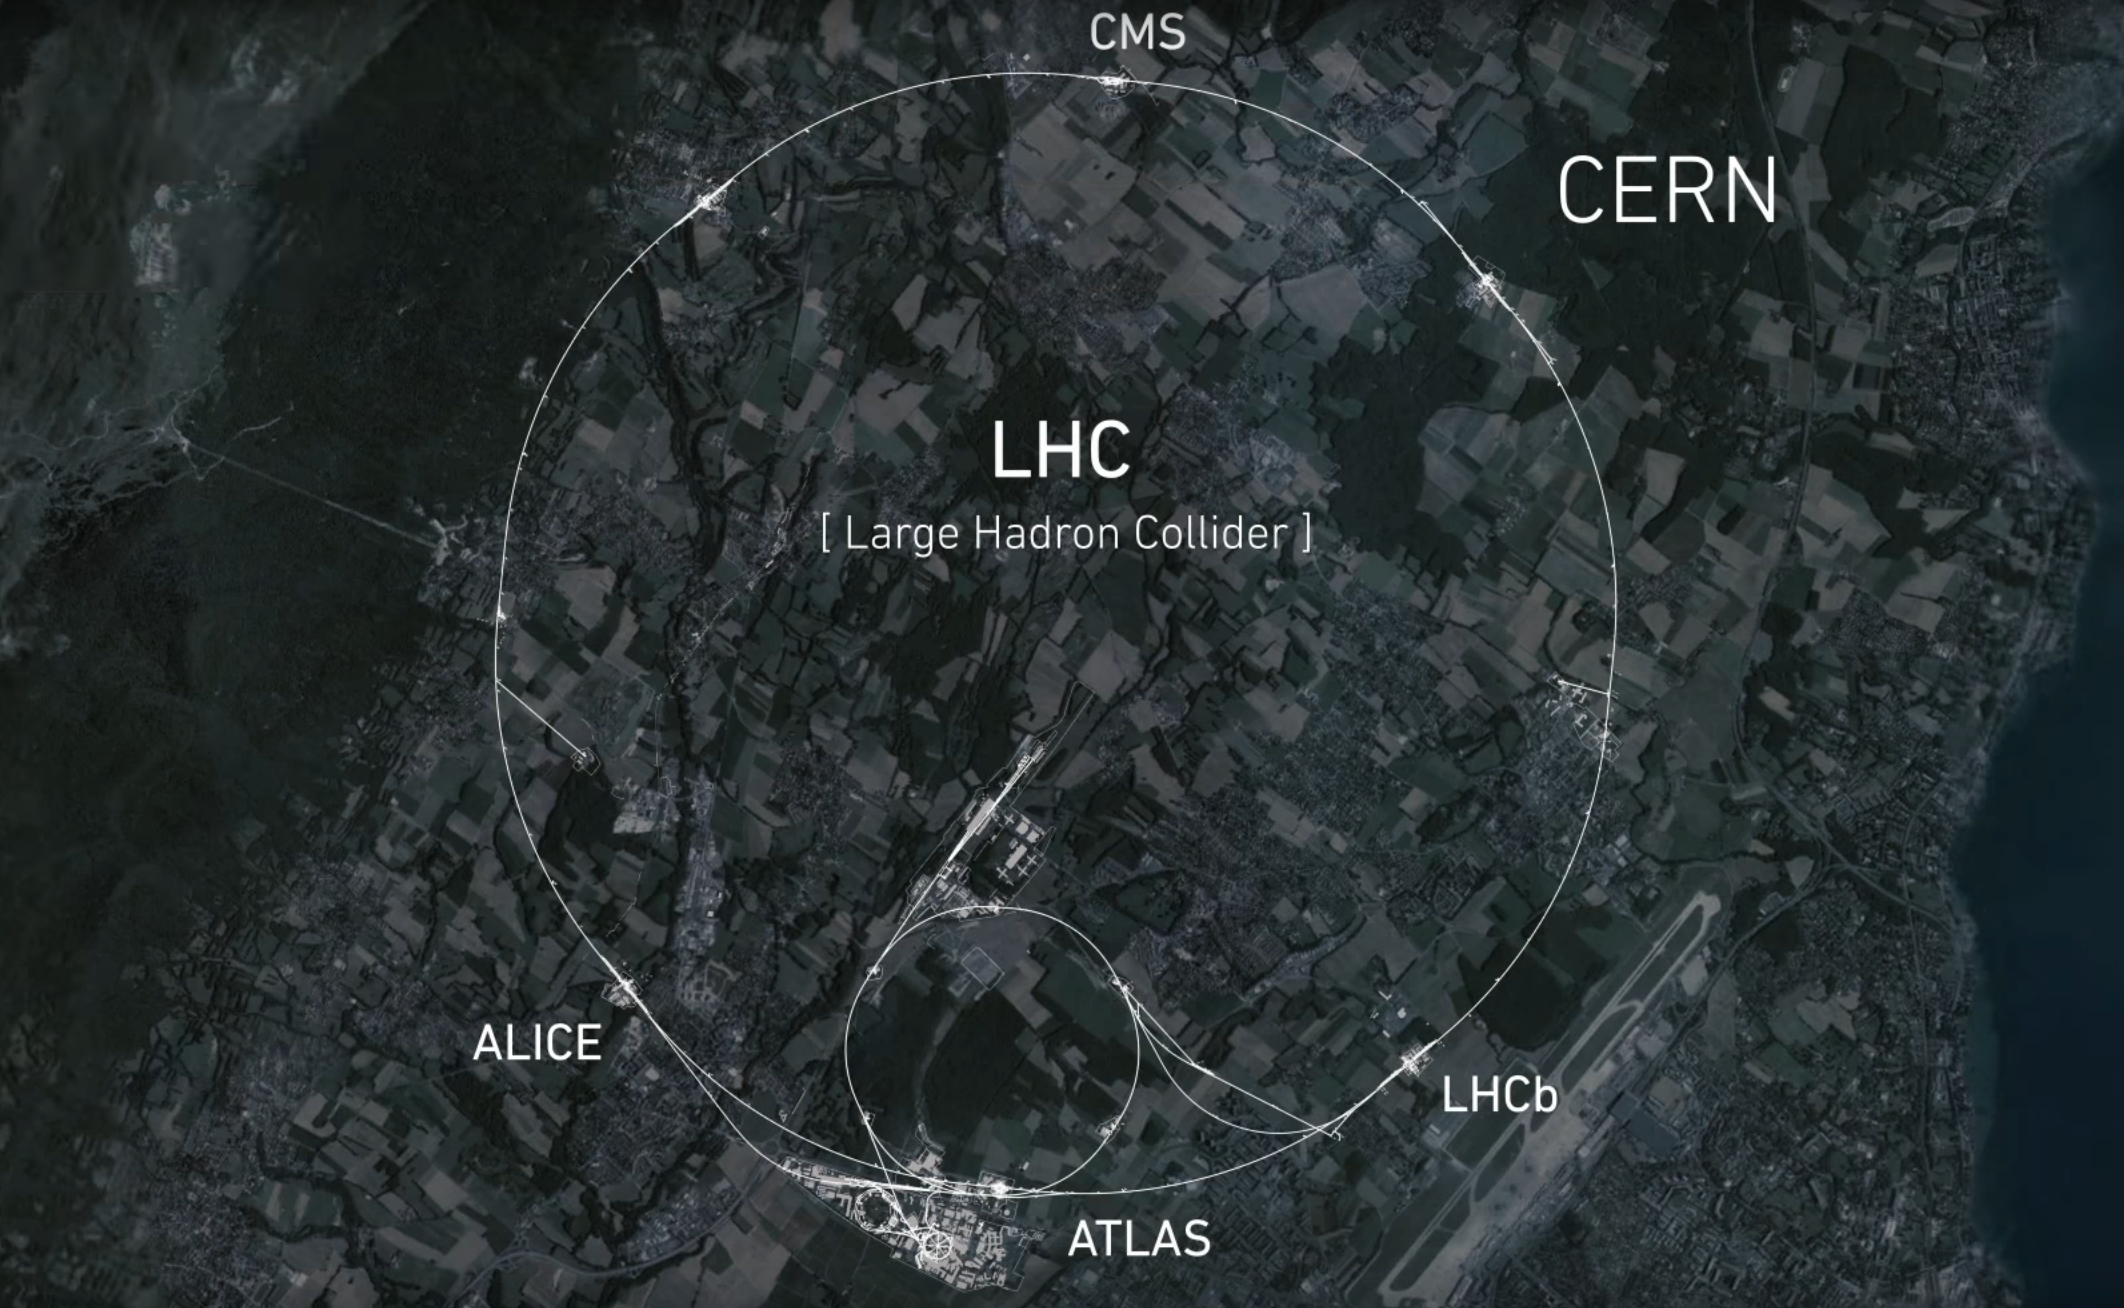
\includegraphics[height=6.65cm]{\PhDthesisdir/plots_and_images/CERN_and_LHC/LHC_map2.png}};
\draw [ultra thick, ltcolorred] (5.65,3.6) circle (3) ; %LHC
%\draw [ultra thick, ltcolorred] (5.325,1.375) circle (.775) ; % SPS
%\draw [ultra thick, ltcolorred] (5.025,0.34) circle (.075) ; % PS
%\fill [ltcolorred] (4.925,0.375) circle (.025) ; % Booster
%\draw [thick, ltcolorred] (4.925,0.375) --+ (-85:.1) ; % LINAC2
\end{tikzpicture}
\end{center}
\end{frame}